\chapter{Proposta}
\label{chapter:Proposta}

A seguir, será apresentado cada ponto proposto em tópicos mais detalhados. Dessa forma, o capitulo está organizado visando apresentar a visão geral do \textit{framework} proposto, enfatizado como o mesmo será utilizado; a prova de conceito desenvolvida no intuito de avaliar a adequação de algumas soluções tecnológicas ao tema em investigação, e alguns trabalhos relacionados.

Ao final deste capítulo, pretende-se que o leitor forme uma ideia mais concreta sobre a proposta deste trabalho.

\section{O Framework}

A proposta deste trabalho é desenvolver um \textit{framework} que auxilie no desenvolvimento de redes sociais. Este \textit{framework} deve oferecer recursos gerais com toda a lógica de usuários e relacionamentos, e recursos mais específicos para redes sociais baseadas em rotas e agendas. O recurso de rotas deve ser capaz de fazer um mapeamento de rotas de interesse de um determinado usuário e auxiliar este a fazer comparações com rotas de outros usuários. A agenda deve oferecer recursos de controle de ocupações no decorrer de dias e horários e auxiliar um usuário a encontrar dias e/ou horários comuns entre um grupo de usuários qualquer.

Parte do \textit{framework} será extensível, possibilitando ao desenvolvedor reutilizá-lo a partir de seus pontos flexíveis, modelados e implementados usando o conceito de herança. O desenvolvedor poderá, portanto, acrescentar e/ou alterar suas implementações conforme as suas necessidades. O \textit{framework}, por si só, oferecerá recursos que poderão ser reutilizados diretamente pelo desenvolvedor, não necessitando estendê-los. A extensibilidade só será necessária, caso sejam desejados níveis de especificidade maiores.

A seguir, têm-se um maior detalhamento de cada um dos três principais componentes fornecidos pelo \textit{framework}.

\subsection{Relacionamento de Usuários}

O relacionamento em redes sociais dá-se por meio de interações entre os usuários. Estas interações variam de acordo com a rede em que o usuário está inserido. Alguém pode apenas seguir outras pessoas e acompanhar suas postagens. Este é um relacionamento unidirecional, pois não é necessário que uma pessoa seguida acompanhe também postagens de seus seguidores. Existe também outro tipo de relacionamento, onde é necessário que as duas pessoas estejam diretamente ligadas entre si, o que o torna necessariamente bidirecional. Neste tipo, podem ser considerados relacionamentos entre conhecidos, amigos, namorados, familiares, entre outros.

Na montagem da estrutura de relacionamentos entre os usuários para redes sociais, é necessário fazer uso de grafos, onde os usuários serão representados como os vértices e os relacionamentos como as arestas. No caso dos relacionamentos unidirecionais, apenas uma aresta é criada. Esta aresta faz uma ligação a partir do vértice do usuário seguidor para o vértice do usuário que este deseja seguir, como pode ser observado na figura \ref{segue}. No caso dos relacionamentos bidirecionais, a ligação deverá ser feita usando-se duas arestas paralelas. É necessário que para ambos os usuários exista uma possibilidade de se chegar ao outro, portanto, deve existir uma aresta que ligue um usuário ``A'' a um usuário ``B'' e uma aresta que ligue o usuário ``B'' ao usuário ``A'', vide a figura \ref{amigo}.

\begin{figure}[!h]
	\centering
	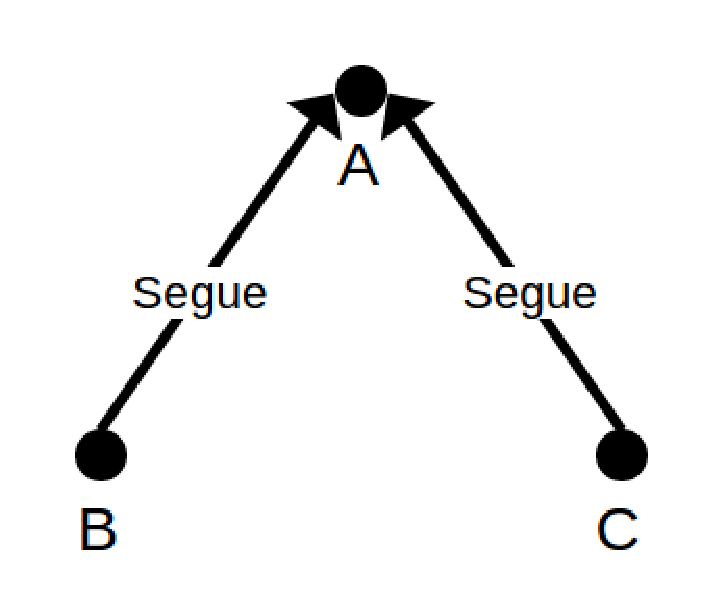
\includegraphics[scale=0.45]{figuras/capitulo5/segue.eps}
	\caption{Exemplo de aresta de seguir usuário}
	\label{segue}
\end{figure}

\begin{figure}[!h]
	\centering
	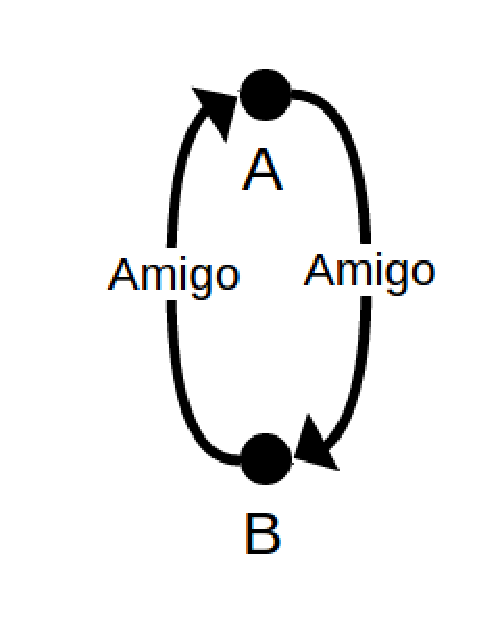
\includegraphics[scale=0.45]{figuras/capitulo5/amigo.eps}
	\caption{Exemplo de arestas paralelas de amizade}
	\label{amigo}
\end{figure}

Cada aresta deverá possuir uma ou mais descrições que detalham qual o relacionamento entre os usuários. Isso fica mais claro ao se falar de relacionamentos bidirecionais, onde pode existir entre duas pessoas um relacionamento de amizade e parentesco, por exemplo. Esse relacionamento pode ser visualizado na figura \ref{parentes}.

\newpage

\begin{figure}[!h]
	\centering
	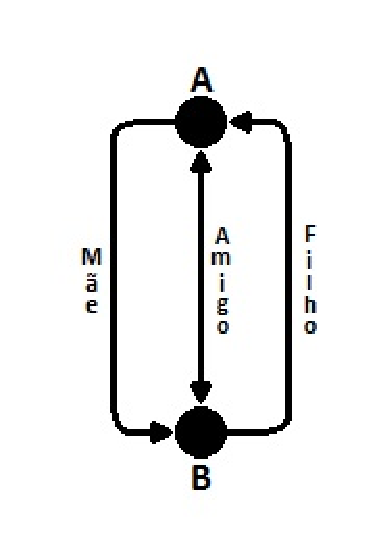
\includegraphics[scale=0.45]{figuras/capitulo5/parentes.eps}
	\caption{Exemplo de arestas paralelas parentesco}
	\label{parentes}
\end{figure}

\subsection{Controle de Rotas}

Rota\footnote{\url{http://www.dicio.com.br/rota/}} é um itinerário que se percorre para ir de um lugar a outro, indicando a direção ou rumo a ser percorrido. Um exemplo de rota pode ser visualizado na figura \ref{rota}.

\begin{figure}[!h]
	\centering
	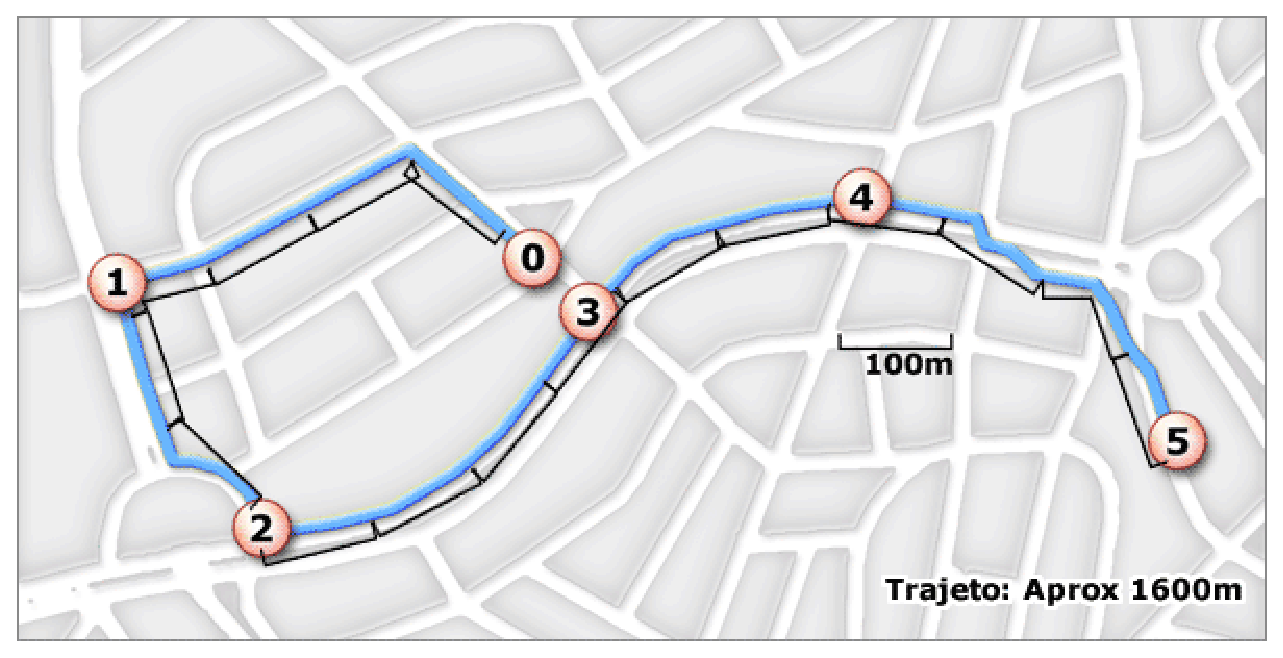
\includegraphics[scale=0.55]{figuras/capitulo5/rota.eps}
	\caption[Exemplo de rota]{Exemplo de rota\footnotemark}
	\label{rota}
\end{figure}
\footnotetext{\url{http://sede.wikidot.com/andy-s-brainstorm}}

O \textit{framework} irá oferecer recursos que auxiliem o usuário a definir as rotas que percorre e os horários de cada percurso, e buscar rotas de outros usuários que coincidam em parte ou integralmente com as suas.

Redes sociais podem utilizar estes dados para aplicações diversas como, por exemplo, caronas e encontros para ciclistas.

Conforme mostrado na figura \ref{rota}, pode-se ver uma rota que leva do ponto ``0'' ao ponto ``5''. Podem existir diversos usuários com rotas comuns nesse caminho, por exemplo, um usuário que siga todo o caminho traçado, ou um usuário que partisse do ponto ``2'' e chegasse ao ponto ``4'' e assim por diante. Uma das funcionalidades do \textit{framework}, neste contexto, seria encontrar todos os usuários que compartilhassem esses caminhos, ou encontrar um caminho compartilhado entre um grupo de usuários, por exemplo.

\subsection{Controle de Agenda}

Outra funcionalidade que o \textit{framework} irá fornecer é a conciliação de agendas entre os usuários, possibilitando assim encontrar dias da semana e horários específicos que são comuns a um determinado grupo. Esta funcionalidade pode auxiliar os usuários em diversos aspectos como, por exemplo, encontrar um horário em comum para realizar uma tarefa.

A figura \ref{agenda semanal} mostra um exemplo de uma agenda semanal com todos os horários livres.

\begin{figure}[!h]
	\centering
	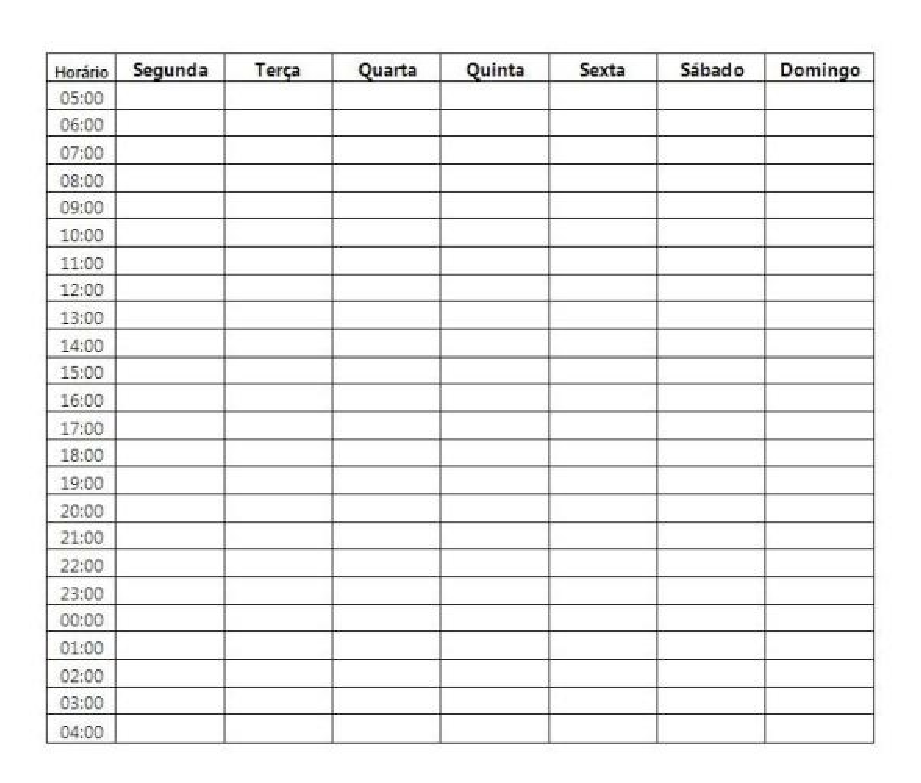
\includegraphics[scale=0.55]{figuras/capitulo5/agenda_semanal.eps}
	\caption[Exemplo de agenda semanal]{Exemplo de agenda semanal\footnotemark}
	\label{agenda semanal}
\end{figure}
\footnotetext{\url{http://universovocesaude.com.br/wp-content/uploads/2014/08/horario-semanal_JPG.jpg}}

Agendas dessa forma auxiliam usuários a terem um melhor controle de suas tarefas semanais, marcarem eventos, entre outros aspectos. O período compreendido por uma agenda pode variar de acordo com cada contexto. Pode ser uma agenda semanal, conforme a apresentada, mensal, anual, ou ainda um período não necessariamente pré-definido, o que poderia auxiliar usuários a marcarem eventos para longas datas futuras. De modo simplificado, basta dados como dia e horários de início e fim de uma tarefa para aplicar um controle de agenda.

O \textit{framework} oferecerá o suporte para criação de agendas conforme apresentado. Assim, é possível a partir de um período pré-determinado encontrar um horário e dia comuns a um conjunto de usuários. Isso pode auxiliar a criação e marcação de eventos visando atender o maior número de usuários, conforme o contexto da aplicação.

\subsection{Modelo Inicial}

A figura \ref{diagrama de componentes} apresenta os principais componentes que serão oferecidos pelo \textit{framework}. Fica evidenciado, no modelo, o relacionamento de usuário com rotas e agendas. Em cada um desses componentes, existirão diversas classes que implementarão todo o modelo e as regras de negócio propostas.

\begin{figure}[!h]
	\centering
	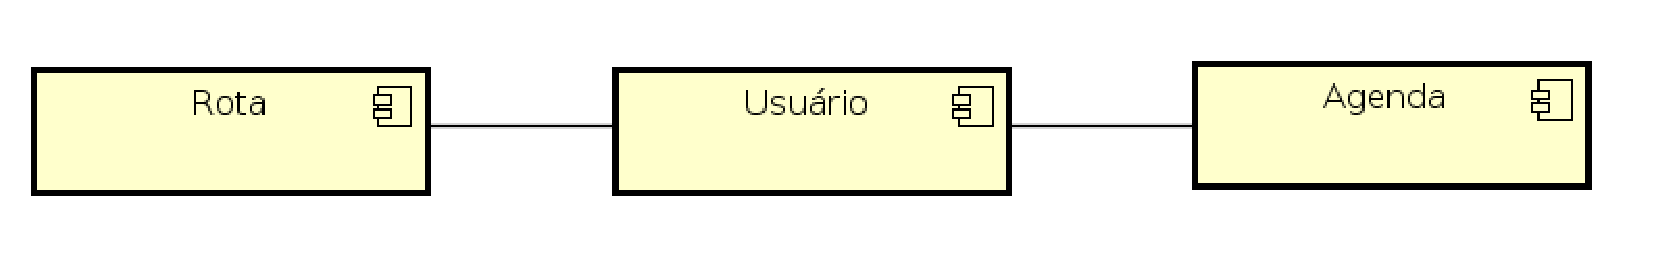
\includegraphics[scale=0.55]{figuras/capitulo5/diagrama_componentes.eps}
	\caption{Diagrama de componentes inicial}
	\label{diagrama de componentes}
\end{figure}

O diagrama mostra apenas um modelo preliminar que dará base para a implementação das funcionalidades propostas. Cada componente conterá diversos algoritmos relacionados e aplicará padrões de projetos que se encaixem, buscando a melhor qualidade, soluções reutilizáveis e fácil manutenção e evolução.

\section{Uso do Framework}

O \textit{framework} será desenvolvido em \textit{``Ruby on Rails''} e terá sua \textit{``Gem''}\footnote{\url{httpttp://www.akitaonrails.com/2009/2/2/entendendo-rubygems}} publicada em um repositório \textit{online} para uso de outros desenvolvedores.

Para comprovação do funcionamento do \textit{framework}, este trabalho propõe o desenvolvimento de uma rede social que faça uso do mesmo. Esta rede deverá fazer uso dos principais recursos providos pelo \textit{framework}. Dessa forma, será possível avaliar o seu uso na prática.

A figura \ref{uso_proposto} apresenta um modelo que procura ilustrar e contextualizar um possível uso para o \textit{framework}.

\begin{figure}[!h]
	\centering
	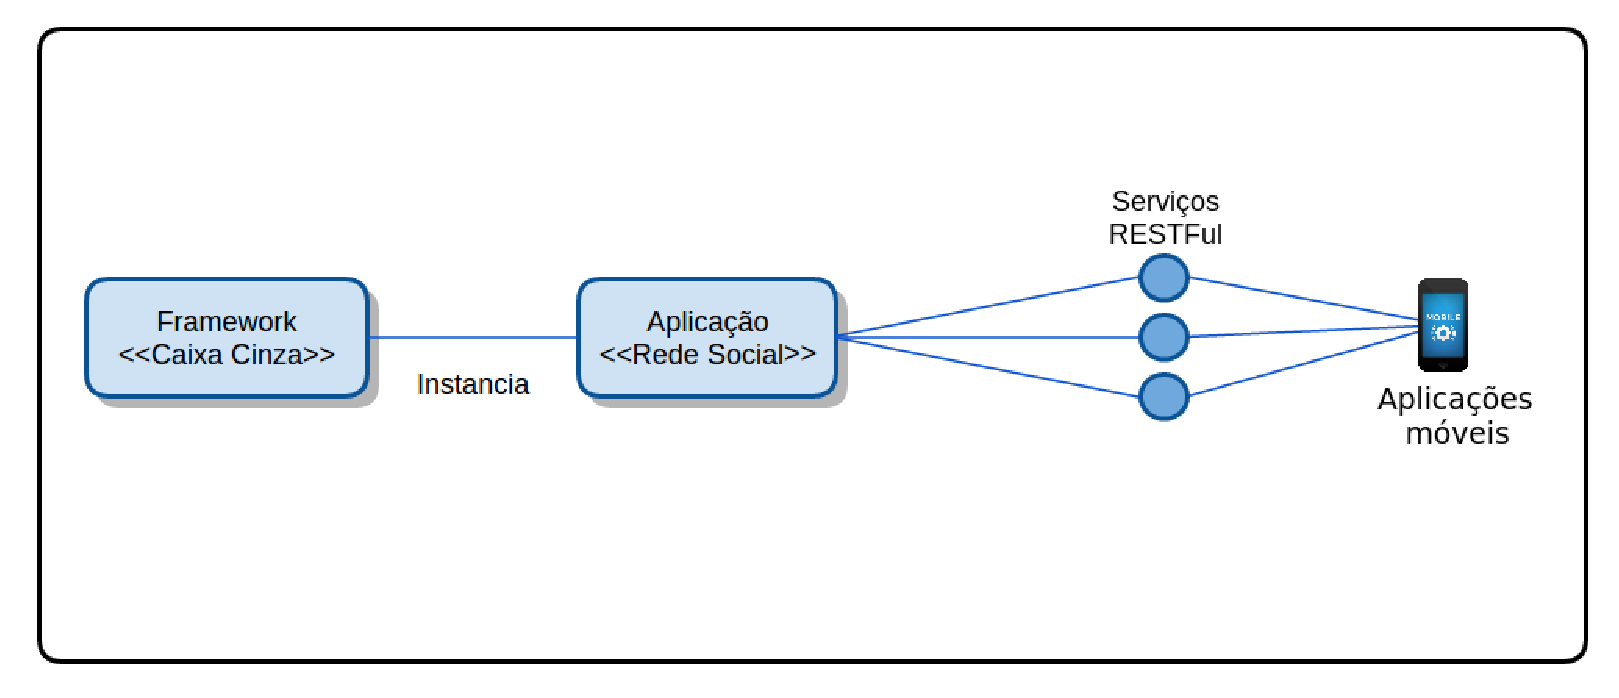
\includegraphics[scale=0.45]{figuras/capitulo5/uso_proposto.eps}
	\caption{Modelo ilustrando um possível uso do \textit{Framework}}
	\label{uso_proposto}
\end{figure}

O modelo apresentado na Figura \ref{uso_proposto} mostra a instanciação do \textit{framework}  visando o desenvolvimento de uma rede social. Essa instanciação traz consigo toda a implementação desenvolvida no \textit{framework} e a disponibiliza para ser usada na aplicação. Ao analisar a Figura \ref{uso_proposto}, percebe-se um \textit{framework} \textit{``black box''}. Entretanto, a real proposta apresenta um \textit{framework} \textit{``grey box''}, pois, grande parte das classes disponibilizadas podem ser estendidas e ter os métodos alterados, ou atributos acrescentados, entre outros aspectos. Ressalta-se ainda, que os componentes mostrados no diagrama na seção anterior são disponibilizados como pacotes na forma de \textit{hotspots} \cite{Franca:2001} garantindo, assim, uma maior flexibilidade ao desenvolvedor na escolha dos componentes que serão utilizados. O \textit{framework} possui como \textit{frozenspots} \cite{Franca:2001} a sua estrutura de relacionamento entre as classes principais e os algoritmos de varredura em grafos ~\nameref{subsec:bfs} e ~\nameref{subsec:dfs}.

Seguindo ainda o modelo na Figura \ref{uso_proposto}, é indicado o uso de serviços \textit{RESTFul} para a aplicação desenvolvida. Esses serviços reforçam mais uma vez a ideia de reutilização de software ao fornecerem recursos simples e leves para utilização em dispositivos móveis, por exemplo, sem a necessidade de replicação da lógica de negócio desenvolvida por trás da aplicação. Contudo, esse é um uso recomendado, e cabe ao desenvolvedor disponibilizar esses serviços em sua rede social.

\section{Prova de Conceito}

Foi desenvolvida uma pequena aplicação para implementação de alguns conceitos discutidos neste trabalho.

De modo geral, a aplicação desenvolvida implementa uma rede de usuários ligados entre si formando um grafo. A solução contêm as classes Usuário, Aresta e Grafo. A classe Aresta é usada para fazer as ligações entre as entidades. A classe Grafo representa a própria rede com todos os usuários. A classe de Usuário pode ser vista como os vértices do grafo. Foram implementadas as funcionalidades de relacionamento descritas nas figuras \ref{segue} e \ref{amigo}, além de uma varredura dos usuários presentes no grafo pelos algoritmos de busca ~\nameref{subsec:bfs}, \textit{Breadth-First Search}, e ~\nameref{subsec:dfs}, \textit{Depth-First Search}.

A figura \ref{modelo prova de conceito} apresenta o modelo das classes desenvolvidas na aplicação de prova de conceito e seus respectivos relacionamentos.

\begin{figure}[!h]
	\centering
	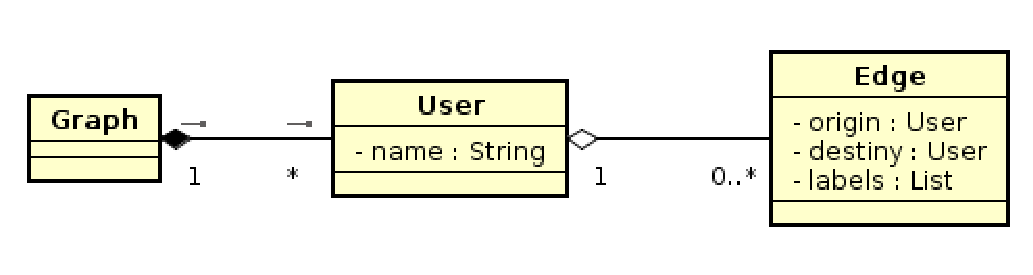
\includegraphics[scale=0.8]{figuras/capitulo5/classes_prova_conceito.eps}
	\caption{Classes da prova de conceito}
	\label{modelo prova de conceito}
\end{figure}

Fica exemplificado o relacionamento entre as classes Grafo e Usuário na forma de uma composição, que indica que um usuário não pode existir sem estar presente na rede. O relacionamento dos usuários, como pode ser visto na figura, é feito através das arestas que possuem: (i) um atributo origem, que representa de qual usuário parte o relacionamento e (ii) um atributo destino, que representa a qual usuário é indicado o relacionamento criado. Cada aresta possui ainda uma lista de \textit{labels} que representam os nomes dos relacionamentos entre os usuários.

Pode-se ver ainda na figura a apresentação dos métodos construídos. A classe user possui os métodos responsáveis por fazer os relacionamentos entre usuários, conforme apresentado nas figuras \ref{segue} e \ref{amigo}. O método \textit{``follow\_user''} é responsável por criar um relacionamento unidirecional, que representa seguir um usuário. O método \textit{``add\_friend''} é responsável por relacionamentos bidirecionais. Este último, por sua vez, necessita ainda ser complementado pelo método \textit{``confirm\_friend''}, pois, ao se invocar o método \textit{``add\_friend''} cria-se uma aresta que possui o \textit{label} amigo e pendente, o que indica que o relacionamento ainda não está completo. Ao se invocar o método \textit{``confirm\_friend''}, outra aresta é criada no outro sentido e o \textit{label} pendente é removido, completando-se assim, o relacionamento entre os dois usuários.

A classe grafo possui o método \textit{``add\_user''}, que é chamado sempre na criação de um novo usuário, visando adicionar este a rede. O método \textit{``set\_white''} tem como objetivo definir a cor de todos os usuários no grafo para branco. Esse atributo é usado ao se trabalhar com os recursos de buscas no grafo. Colorir o nó com a cor branca significa que este ainda não foi visitado. O método \textit{``dfs''} implementa o algoritmo de busca ~\nameref{subsec:dfs} e faz uma varredura no grafo. O mesmo acontece para o método \textit{``bfs''} que implementa a varredura de acordo com o algoritmo \textit{``bfs''}. Os métodos \textit{``dfs\_visit''} e \textit{``bfs\_visit''} são métodos auxiliares que visitam o nó corrente e definem o próximo nó que será visitado de acordo com as regras definidas nos algoritmos.

A abordagem de lista de adjacência foi utilizada na implementação do grafo. Como as arestas trabalhadas possuem outras informações além da representação das ligações entre os nós, essa abordagem ocupa menos espaço. Isso ocorre, pois não existe representação de arestas que não estejam presentes no grafo. Além da redução da memória gasta, torna-se mais fácil encontrar os nós que fazem ligação a um outro nó, quando se usa lista de adjacência, pois basta realizar a leitura da lista para se obter essas informações. Já na matriz de adjacência e incidência, é necessário realizar uma busca na matriz para verificar as ligações que um nó possui.

Todo o código fonte da aplicação citada pode ser encontrado em \url{https://github.com/TCC-SocialNetwork/concept-test}.

Essa aplicação representa a prova de conceito visando entender detalhes básicos de redes sociais, e compreender as reais dificuldades para o pleno desenvolvimento do \textit{framework} proposto. Essa prova de conceito procura lidar com uma funcionalidade chave em redes sociais, no caso, o relacionamento de usuários. Portanto, é vista como um passo inicial para o desenvolvimento da proposta. O desenvolvimento completo será realizado na segunda parte deste trabalho, conforme evidenciado no fluxo de trabalho bem como no cronograma, ambos apresentados no capítulo de ~\nameref{chapter:Metodologia}.

\section{Trabalhos Relacionados}

Em algumas pesquisas relacionadas sobre trabalhos parecidos com o que se propõe, pode-se encontrar alguns sistemas semelhantes, os quais serão apresentados a seguir.

Existe uma comparação entre vinte e cinco plataformas, as quais colaboram para começar um serviço de rede social\footnote{\url{http://www.tripwiremagazine.com/2010/07/25-best-social-networking-platforms-to-start-your-own-service.html}}  próprio. Porém, algumas das plataformas apresentadas são pagas ou não são voltadas para desenvolvedores, ou seja, são plataformas que fornecem funcionalidades para usuários comuns poderem montar uma rede social a partir de um \textit{template} visual já definido.

A Tabela \ref{comparacao} apresenta um comparativo entre algumas das plataformas que apresentam suporte à criação de redes sociais. Durante a pesquisa realizada para constatar as características de cada plataforma, percebeu-se que as plataformas feitas a partir da linguagem de programação PHP são predominantes. Porém, no intuito de focar nas plataformas que fornecem suporte para outras linguagens, foram apresentadas apenas cinco das plataformas que fornecem suporte ao PHP, dando assim um maior enfoque nos diferentes tipos de linguagens.

Uma outra característica importante que foi observada na comparação é que os componentes customizáveis que as plataformas afirmam possuir são, em sua maioria, via interface gráfica. Em poucas plataformas é possível a customização via código, sendo, nesses casos, a maior parte feita via construção de \textit{plugins}.

\newpage

\begin{table}[]
\centering
\caption{Comparação entre os trabalhos relacionados}
\label{comparacao}
\begin{adjustbox}{width=\textwidth}
\begin{tabular}{@{}llllll@{}}
\toprule
\textbf{Rede Social}  & \textbf{Licença} & \textbf{Preço}        & \textbf{Linguagem}  & \textbf{Customizável}                                    \\ \midrule
SocialEngine          & Customizada      & A partir de \$ 299,99 & PHP                 & Sim                                                      \\
Elgg                  & GPL 2.0          & Grátis                & PHP                 & Extensível via plugins e com uma API flexível            \\
XOOPS                 & GPL 2.0          & Grátis                & PHP                 & Extensível via módulos                                   \\
mooSocial             & Customizada      & A partir de \$ 149,99 & PHP                 &                                                          \\
Anahita Social Engine & GPL 2.0          & Grátis                & PHP                 & Sim                                                      \\
Telligent Community   & Customizada      & Grátis com limitações & ASP .NET            & Extensível via plugins, widgets, tarefas, eventos e REST \\
Newebe                & AGPL             & Grátis                & Python/Coffeescript & Sim                                                      \\
Buddycloud            & Apache 2.0       & Grátis                & NodeJS/Java         & Sim                                                      \\
eXo Platform          & LGPL             & Grátis                & Java                & Extensível via plugins e com uma API flexível            \\
Kune                  & AGPLv3           & Grátis                & Java                & Extensível via widgets e módulos                         \\
Diaspora              & AGPLv3           & Grátis                & Ruby                & Sim                                                      \\
Insoshi               & MIT              & Grátis                & Ruby                & Sim                                                      \\
Libertree             & AGPLv3           & Grátis                & Ruby                & Sim                                                      \\ \bottomrule
\end{tabular}
\end{adjustbox}
\end{table}

Existem também alguns \textit{frameworks} mais semelhantes desenvolvidos em \textit{Ruby}\footnote{\url{https://www.ruby-toolbox.com/categories/social_networking}}. Estes, em sua maioria, fornecem recursos a desenvolvedores, porém apenas a parte geral de relacionamento de usuários. A seguir é possível visualizar na Figura \ref{ruby_social_network} uma comparação da popularidade desses \textit{frameworks}. O cálculo da popularidade é feito com base na quantidade de observadores e de \textit{forks} que o repositório do \textit{framework} possui.

\begin{figure}[!h]
	\centering
	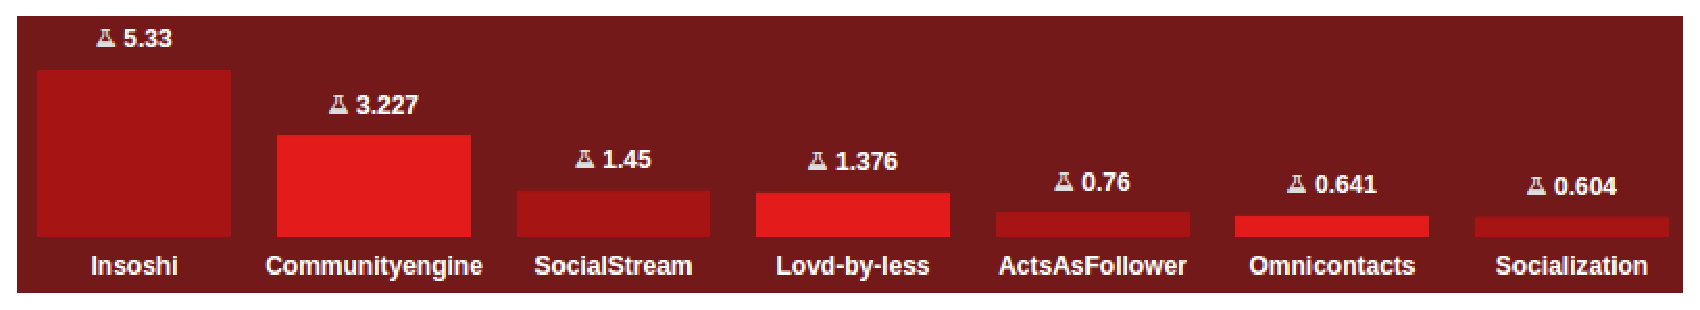
\includegraphics[scale=0.45]{figuras/capitulo5/ruby_social_network.eps}
	\caption{Popularidade dos \textit{Frameworks} em \textit{Ruby}}
	\label{ruby_social_network}
\end{figure}

\section{Resumo do Capítulo}

Este capítulo descreveu a proposta deste trabalho apresentando seus pontos principais e alguns detalhes técnicos.

A partir desse escopo inicial, pretende-se desenvolver um \textit{framework}  capaz de auxiliar interessados no desenvolvimento de redes sociais, das funcionalidades básicas às específicas dos domínios de rota e agenda. Dando continuidade aos resultados obtidos até o momento, com a prova de conceito, serão elaborados os requisitos detalhados para construção do \textit{backlog} do produto e, a partir desse, a definição das \textit{sprints} e \textit{releases} que orientarão o desenvolvimento.

O próximo capítulo fecha este documento com uma conclusão parcial de todo o trabalho feito até o presente momento. Este capítulo deverá ser incrementado após a finalização da etapa de desenvolvimento do \textit{framework}.
